\section{Pendahuluan}
\subsection{Latar Belakang}
Perkembangan teknologi jaringan komputer yang pesat telah menyebabkan kebutuhan akan sistem pengalamatan yang lebih luas dan efisien. Protokol IPv4 yang selama ini digunakan memiliki keterbatasan dalam jumlah alamat yang dapat diberikan, serta tidak dirancang untuk menangani kebutuhan komunikasi modern yang semakin kompleks, seperti mobilitas perangkat, keamanan, dan efisiensi routing. Untuk mengatasi keterbatasan ini, IPv6 diperkenalkan sebagai generasi penerus dari IPv4. \\ IPv6 menawarkan ruang alamat yang sangat besar, fitur auto-configuration, peningkatan keamanan dengan IPsec, serta manajemen jaringan yang lebih efisien. Namun, penerapan dan pengelolaan jaringan berbasis IPv6 membutuhkan pemahaman yang mendalam mengenai konfigurasi alamat, routing, dan manajemen perangkat dalam jaringan tersebut. \\ Modul ini disusun sebagai panduan praktis dalam memahami proses routing dan manajemen jaringan menggunakan IPv6. Pembahasan mencakup konfigurasi alamat IPv6 pada interface, pengelolaan routing statis, serta penggunaan command-line interface (CLI) untuk observasi dan pemecahan masalah.

\subsection{Dasar Teori}
IPv6 adalah versi terbaru dari protokol internet yang dirancang untuk menggantikan IPv4. IPv6 menggunakan panjang alamat 128-bit memungkinkan lebih dari 340 undecillion alamat unik. Ini mengatasi keterbatasan jumlah alamat pada IPv4 yang hanya menggunakan 32-bit. \\ Alamat IPv6 dituliskan dalam notasi heksadesimal, dipisahkan oleh titik dua (:), dan terdiri dari delapan kelompok. Ada beberapa jenis alamat IPv6, antara lain Unicast (Mengidentifikasi satu antarmuka tunggal), Multicast (Mengidentifikasi sekelompok antarmuka), Anycast (Alamat yang dapat digunakan oleh beberapa antarmuka tetapi dikirimkan ke yang terdekat). \\ Routing dalam jaringan IPv6 melibatkan pengiriman paket dari satu jaringan ke jaringan lain berdasarkan alamat tujuan IPv6. Routing dapat bersifat statis dan dinamis. \\ IPv6 menggunakan NDP sebagai pengganti ARP (Address Resolution Protocol) pada IPv4. NDP digunakan untuk mendeteksi tetangga, menemukan router, serta mengelola informasi tentang alamat link-local dan konfigurasi jaringan lainnya. \\ Konfigurasi alamat dan routing IPv6 dilakukan melalui CLI seperti pada sistem operasi Linux menggunakan perintah seperti ip, ping6, dan ip -6 route. Manajemen jaringan juga melibatkan pengaturan interface, pengecekan konektivitas, serta pemantauan tabel routing.

%===========================================================%
\section{Tugas Pendahuluan}
\begin{enumerate}
	\item IPv6 (Internet Protocol version 6) adalah versi terbaru dari protokol Internet yang dirancang untuk menggantikan IPv4. IPv6 menggunakan alamat 128-bit, yang memungkinkan penyediaan jumlah alamat IP yang sangat besar, sekitar 340 triliun triliun triliun alamat unik. Ini sangat berbeda dengan IPv4 yang hanya menyediakan sekitar 4,3 miliar alamat IP karena menggunakan alamat 32-bit. \\ IPv6 dikembangkan oleh Internet Engineering Task Force (IETF) sebagai solusi atas keterbatasan jumlah alamat IPv4 yang semakin menipis akibat pertumbuhan pesat perangkat yang terhubung ke internet. Selain kapasitas alamat yang sangat besar, IPv6 juga membawa sejumlah fitur baru seperti efisiensi routing yang lebih baik, keamanan yang lebih tinggi, dan dukungan otomatisasi konfigurasi jaringan. \\ IPv6 menyediakan ruang alamat yang jauh lebih besar dibandingkan IPv4. IPv4 menggunakan format numerik desimal, sedangkan IPv6 menggunakan kombinasi angka dan huruf heksadesimal yang dipisahkan titik dua. Pv4 mengenal broadcast, sedangkan IPv6 menggantinya dengan anycast dan multicast, yang lebih efisien dalam pengiriman data ke banyak tujuan.
	\item A. Subnet A : 2001:db8:0000:0000::/64 \\ Subnet B : 2001:db8:0000:0001::/64 \\ Subnet C : 2001:db8:0000:0002::/64 \\ Subnet D : 2001:db8:0000:0003::/64 \\\\ B. Subnet A : 2001:db8:0:0::/64 \\ Subnet B : 2001:db8:0:1::/64 \\ Subnet C : 2001:db8:0:2::/64 \\ Subnet D : 2001:db8:0:3::/64
	\item ether 1 : 2001:db8:0:0::1/64 \\ ether 2 : 2001:db8:0:1::1/64 \\ ether 3 : 2001:db8:0:2::1/64 \\ ether 4 : 2001:db8:0:3::1/64
	\item Ip table 
	\begin{figure}[H]
		\centering
		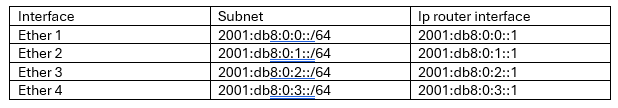
\includegraphics[width=0.65\linewidth]{image/ip table.png}
		\label{fig:inirujukan}
	\end{figure}
	\item Routing statis pada jaringan IPv6 adalah metode di mana administrator jaringan secara manual menambahkan entri rute ke dalam tabel routing router. Dengan kata lain, administrator menentukan secara eksplisit jalur mana yang harus dilalui paket data untuk mencapai jaringan tujuan tertentu, beserta gateway yang digunakan. Fungsi utama routing statis yaitu : \\ 1. Memberikan kontrol penuh kepada administrator terhadap jalur lalu lintas jaringan. \\ 2. Membatasi dan mengatur arus lalu lintas secara presisi, sehingga dapat mengoptimalkan keamanan dan efisiensi jaringan. \\ 3. Mencegah kesalahan pengiriman paket data dengan menentukan rute secara spesifik. \\ 4. Mengurangi beban kerja router karena tidak perlu menjalankan protokol routing dinamis yang memerlukan pertukaran informasi dan perhitungan topologi secara terus-menerus. \\ 5. Sangat berguna untuk jaringan kecil atau jaringan dengan topologi yang jarang berubah, karena konfigurasi dan pemeliharaannya lebih sederhana serta lebih dapat diandalkan. \\ Routing statis lebih cocok digunakan pada kondisi Ketika jumlah router dan rute yang harus dikonfigurasi masih sedikit, sehingga penambahan atau perubahan rute dapat dikelola secara manual tanpa membebani administrator jaringan. 
\end{enumerate}